\documentclass[11pt,a4paper]{article} 
\usepackage[portuges]{babel}
\usepackage[utf8]{inputenc}
\usepackage{graphicx}
\usepackage{listings}
\usepackage{amsthm}
\usepackage{booktabs}
\usepackage{amsfonts}
\usepackage{subcaption}
\usepackage[table,xcdraw]{xcolor}
\graphicspath{{..//images//}}

\title{Física Geral - Relatório de prática - Lei de Ohm}
\author{Juliana Cavalcanti Correa}


\begin{document}
   
  \maketitle

  \section{Esquema experimental}
  \label{sec:esquema}
    
    \paragraph{}
    Nesta prática, o objetivo é verificar experimentalmente a Lei de Ohm. Para isso, foi usado  um circuito contendo apenas elementos resistivos dentro da faixa de operação ôhmica, isto é, cuja resistência deve ser constante. Nesse caso, a lei afirma que a razão entre a tensão no circuito e a corrente que circula por ele é dada pela resistência equivalente de seus elementos.
    \paragraph{}
    Para essa verificação, a prática foi dividida em duas etapas. Na primeira, foram tomadas medidas diretas da resistência usando dois resistores em quatro arranjos diferentes - cada um dos dois individualmente, os dois em série e os dois em paralelo. Já na segunda etapa, foram aplicadas tensões com valores entre 2V e 20V sobre os mesmos arranjos de resistores e efetuada a medição da corrente correspondente a cada valor de tensão. Os esquemas de montagem no \textit{protoboard} podem ser visualizados na Figura ~\ref{fig:esquemas}.
    \paragraph{}
    Os valores teóricos das resistências podem ser calculados através do código de cores apresentados nos resistores. Os dois utilizados tinham o mesmo código, indicando resistência nominal de $10k\Omega\pm 5\%$. 
    \paragraph{}
    No arranjo em série, a corrente que atravessa os dois resistores é a mesma, por isso a resistência equivalente prevista pela Lei de Ohm é a soma das duas resistências, visto que $V = R_{eq} \cdot i = R_{1} \cdot i + R_{2} \cdot i$. A $R_{eq}$ prevista nesse caso é, então, de $20k\Omega$.
    \paragraph{}
    Já no arranjo em paralelo, a tensão aplicada sobre os dois resistores é a mesma, fazendo com que a corrente se divida entre os dois resistores. Portanto, a corrente total é a soma  das correntes nos dois resistores e a Lei de Ohm prevê que $\frac{V}{R_{eq}} = \frac{V}{R_{1}} + \frac{V}{R_{2}}$. Para os dois resistores usados, a $R_{eq}$ em paralelo vale $5k\Omega$.
      
    \begin{figure}[htb!]
      \centering
      \captionsetup{justification=centering}  
      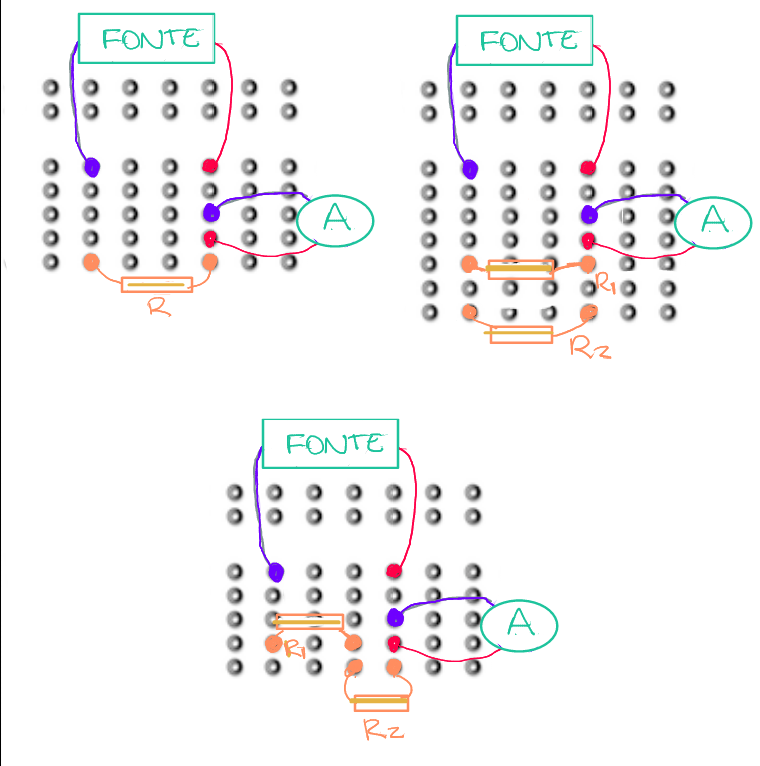
\includegraphics[scale=0.45]{esquemas2.png}
      \caption{Esquemas de montagem. Acima, à esquerda, somente um resistor; à direita os dois resistores em paralelo; abaixo, os dois resistores em série.}
      \label{fig:esquemas}
    \end{figure}

  \section{Procedimento experimental}

      \paragraph{}
      Na etapa preliminar, foram usados um multímetro analógico e um digital para medir a resistência equivalente dos quatro arranjos descritos. Com cada um dos dois instrumentos, foram tomadas dez medidas de cada arranjo, para garantir que os resistores estavam operando normalmente, o que de fato foi constatado - para todos os casos, as dez medições foram iguais. Esses valores estão resumidos na Tabela ~\ref{tab:diretas}, junto com os valores teóricos esperados, conforme descritos na Seção ~\ref{sec:esquema}.
      \paragraph{}
      Para calcular o erro das medidas, deveríamos combinar o erro estatístico com o erro do instrumento, porém, como todas as medidas de cada conjunto foram idênticas, não foi possível calcular o erro estatístico. Dessa forma, o erro de cada medida é o erro do instrumento, que, segundo os manuais dos fabricantes, no multímetro analógico vale 4\% e no digital 1,2\%+5d, o que equivale a 0,012*R + 0,05, onde R é a resistência medida, visto que as medidas foram tomadas em uma escala com duas casas decimais de precisão.
      Além disso, para os valores teóricos, o erro de cada resistor, indicado pelos seus códigos de cores, é de $500\Omega = 0,5k\Omega$, e o das combinações é derivado a seguir:
      \begin{itemize}
        \item Erro teórico para os resistores em série (k$\Omega$) = $\sqrt{0,5^{2} + 0,5^{2}}$
        \item Erro teórico para os resistores em paralelo (k$\Omega$) = $5^{2}\cdot(\frac{0,5}{10^{2}}+ \frac{0,5}{10^{2}})$
      \end{itemize} 
         
      \begin{table}[htb!]
        \centering 
        \begin{tabular}{c|cccc}
          \toprule
                               &  R1            &  R2             & série          & paralelo      \\
          \midrule
          teórico (k$\Omega$)  & $10,0\pm0,5 $  & $10,0 \pm 0,5$  & $20,0\pm0,7$   & $5,0\pm0,3$   \\   
          digital (k$\Omega$)  & $9,90\pm 0,17$ & $9,86 \pm 0,17$ & $19,76\pm0,29$ & $4,94\pm0,11$ \\
          analógico (k$\Omega$)& $8,0\pm0,32$   & $8,0\pm0,32$    & $17,8\pm0,7$   & $4,5\pm0,2$   \\
          \bottomrule
        \end{tabular}
        \caption{Valores esperados e medidas diretas das resistências para os dois tipos de multímetro}
        \label{tab:diretas}
      \end{table}
        
      \paragraph{}
      Na segunda etapa da prática, foram efetuadas dez medidas de corrente para cada arranjo, utilizando uma fonte com valores de tensão com intervalos de 2V, iniciando em 2V e terminando em 20V, de acordo com o esquema descrito na Seção ~\ref{sec:esquema} e os resultados estão sumarizados na Tabela ~\ref{tab:indiretas}.

      \begin{table}[htb!]
        \centering
        \begin{tabular}{c|cccc}
          \toprule
          V (V) & i$_1$(mA) & i$_2$ (mA) & i$_{serie}$ (mA) & i$_{paralelo}$(mA) \\
          \midrule
          2     & 0.214   & 0.209   & 0.105        & 0.41            \\
          4     & 0.414   & 0.413   & 0.208        & 0.84            \\
          6     & 0.617   & 0.61    & 0.308        & 1.23            \\
          8     & 0.828   & 0.818   & 0.415        & 1.65            \\
          10    & 1.033   & 1.018   & 0.514        & 2.06            \\
          12    & 1.236   & 1.222   & 0.618        & 2.48            \\
          14    & 1.445   & 1.429   & 0.722        & 2.88            \\
          16    & 1.65    & 1.631   & 0.821        & 3.3             \\
          18    & 1.85    & 1.831   & 0.923        & 3.71            \\
          20    & 2.08    & 2.05    & 1.03         & 4.12            \\
          \bottomrule
        \end{tabular}
        \caption{Medidas de corrente para os diferentes arranjos com valores de tensão variando de 2 a 20V}
        \label{tab:indiretas}
      \end{table}

  \pagebreak
  \section{Tratamento de dados}

    \paragraph{}
    Para verificar a validade da Lei de Ohm, é necessário realizar um ajuste linear utilizando o método dos mínimos quadrados. O método busca ajustar uma reta no gráfico V x i, de tal forma a minimizar a soma dos quadrados dos resíduos, que seria dada pela expressão $$\sum\limits_{k=1}^{10}[V_k - (a \cdot i_k + b)]^2$$ Se a relação expressa pela Lei de Ohm é válida, o coeficiente angular \textbf{a} deve ser compatível com as medidas diretas e o valor teórico de R, e o coeficiente linear \textbf{b} deve ser compatível com 0.
    \paragraph{}
    Na Tabela ~\ref{tab:mmq} são descritos os coeficientes angular e linear encontrados e seus erros, calculados através das seguintes expressões:
    $$a = \sigma_{iV}/\sigma_{ii}^2$$
    $$b = \bar{V} - R\bar{i}$$
    $$\sigma_{a} = \frac{\epsilon_{y}}{\sigma_{x} \cdot \sqrt{N}}$$
    $$\sigma_{b} = \sigma_{a} \cdot \sqrt{\bar{x^2}}$$
   
    \begin{table}[htb!]
      \centering
      \begin{tabular}{c|c|c|c|c}
        \toprule
                      & 1     & 2     & Série & Paralelo \\
        \midrule
        a (= $R_{eq}$) & 9.69  & 9.81  & 19.5  & 4.86  \\
        $\sigma_{a}$   & 0.03  & 0.02  & 0.04  & 0.01  \\
        b              & -0.01 & -0.02 & -0.05 & -0.02 \\
        $\sigma_{b}$   & 0.04  & 0.03  & 0.02  & 0.02  \\
        $\epsilon_{y}$ & 0.06  & 0.05  & 0.04  & 0.03  \\
        \bottomrule
      \end{tabular}
      \caption{Cálculo dos coeficientes do ajuste linear por mínimos quadrados}
      \label{tab:mmq}
    \end{table} 
    
    \paragraph{}
    Os gráficos de V x i dos quatro arranjos podem ser vistos nas Figuras ~\ref{fig:i1} a ~\ref{fig:ip}. As retas resultantes dos coeficientes calculados pelo ajuste linear são representadas pelas linhas laranjas em cada gráfico, enquanto as linhas azuis mostram as retas V = Ri, sendo R o valor teórico das resistências que haviam sido apresentadas na Tabela ~\ref{tab:diretas}. Visualmente, é possível perceber que as retas estão muito próximas, indicando que o resultado foi satisfatório, porém, para comprovar, devemos calcular a compatibilidade dos valores medidos para os coeficientes.

    \begin{figure}[htb!]
      \centering
      \captionsetup{justification=centering}  
      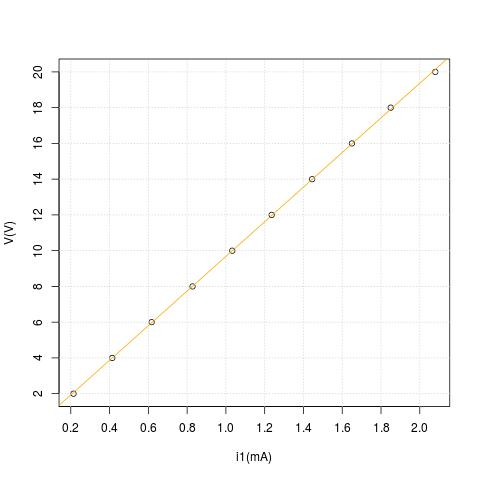
\includegraphics[scale=0.7]{Vi1}
      \caption{Gráfico V x i do resistor 1}
      \label{fig:i1}
    \end{figure}
    
    \begin{figure}[htb!]
      \centering
      \captionsetup{justification=centering}  
      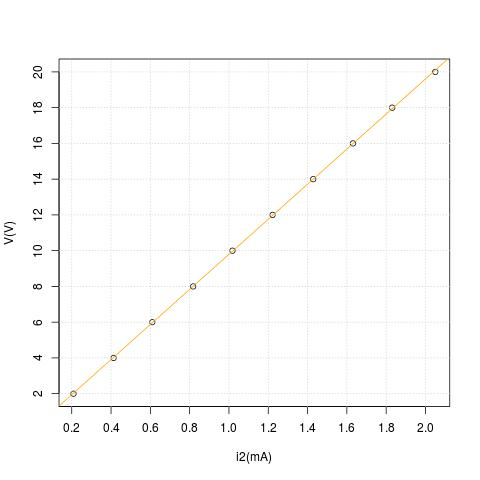
\includegraphics[scale=0.7]{Vi2}
      \caption{Gráfico V x i do resistor 2}
      \label{fig:i2}
    \end{figure}
    
    \begin{figure}[htb!]
      \centering
      \captionsetup{justification=centering}  
      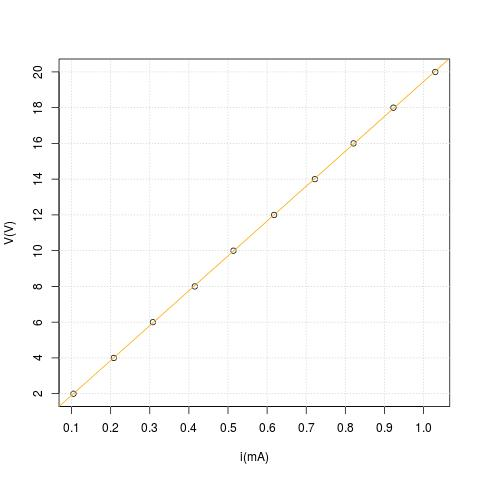
\includegraphics[scale=0.7]{Vis}
      \caption{Gráfico V x i dos resistores em série}
      \label{fig:is}
    \end{figure}
    
    \begin{figure}[htb!]
      \centering
      \captionsetup{justification=centering}  
      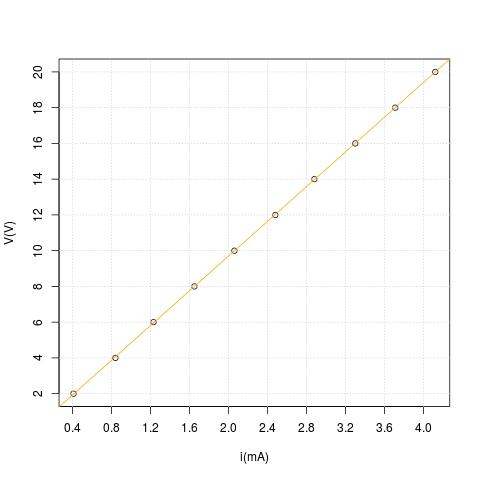
\includegraphics[scale=0.7]{Vip}
      \caption{Gráfico V x i dos resistores em paralelo}
      \label{fig:ip}
    \end{figure}
    
    \clearpage
    \subsection{Cálculo de compatibilidade}
    
      \paragraph{}
      Para verificar a compatibilidade entre cada par de medidas, foram calculadas a discrepância ( $|\bar{x_1}-\bar{x_2}|$ ) e o erro ($\sigma = \sqrt{\sigma_{\bar{x}_1}^2 + \sigma_{\bar{x}_2}^2}$). As medidas são consideradas compatíveis quando a discrepância for menor que 2 vezes o erro. A Tabela ~\ref{tab:compatibilidade} resume a avaliação de compatibilidade.

       \begin{table}[htb!]
        \centering
        \begin{tabular}{llll}
        \toprule
                   & Digital/Teórico   &      &                                     \\
                   & Discrepância      & Erro & Compatível                          \\
          \midrule
          R1       & 0.10              & 0.53 & {\color[HTML]{009901} Sim}          \\
          R2       & 0.14              & 0.53 & {\color[HTML]{009901} Sim}          \\
          série    & 0.24              & 0.76 & {\color[HTML]{009901} Sim}          \\
          paralelo & 0.06              & 0.32 & {\color[HTML]{009901} Sim}          \\
          \midrule
                   & Analógico/Teórico &      &                                     \\
                   & Discrepância      & Erro & Compatível                          \\
          \midrule
          R1       & 2.00              & 0.59 & {\color[HTML]{CB0000} Não}          \\
          R2       & 2.00              & 0.59 & {\color[HTML]{CB0000} Não}          \\
          série    & 2.20              & 0.99 & {\color[HTML]{646809} Inconclusivo} \\
          paralelo & 0.10              & 0.36 & {\color[HTML]{CB0000} Não}          \\
          \midrule
                   & Analógico/Digital &      &                                     \\
                   & Discrepância      & Erro & Compatível                          \\
          \midrule
          R1       & 1.90              & 0.36 & {\color[HTML]{CB0000} Não}          \\
          R2       & 1.86              & 0.36 & {\color[HTML]{CB0000} Não}          \\
          série    & 1.96              & 0.76 & {\color[HTML]{646809} Inconclusivo} \\
          paralelo & 0.04              & 0.23 & {\color[HTML]{009901} Sim}          \\ 
          \midrule
                   & R Calculado/Teórico &      &                                     \\
                   & Discrepância      & Erro & Compatível                          \\
          \midrule
          R1       & 0.31              & 0.50 & {\color[HTML]{009901} Sim}          \\
          R2       & 0.19              & 0.50 & {\color[HTML]{009901} Sim}          \\
          série    & 0.50              & 0.70 & {\color[HTML]{009901} Sim}          \\
          paralelo & 0.14              & 0.20 & {\color[HTML]{009901} Sim}          \\
          \midrule
                   & R Calculado/Medido &      &                                     \\
                   & Discrepância      & Erro & Compatível                          \\
          \midrule
          R1       & 0.21              & 0.17 & {\color[HTML]{009901} Sim}          \\
          R2       & 0.05              & 0.17 & {\color[HTML]{009901} Sim}          \\
          série    & 0.26              & 0.29 & {\color[HTML]{009901} Sim}          \\
          paralelo & 0.08              & 0.11 & {\color[HTML]{009901} Sim}          \\ 
          \midrule
                   & b Calculado/0     &      &                                     \\
                   & Discrepância      & Erro & Compatível                          \\
          \midrule
          R1       & 0.01              & 0.04 & {\color[HTML]{009901} Sim}          \\
          R2       & 0.02              & 0.03 & {\color[HTML]{009901} Sim}          \\
          série    & 0.05              & 0.02 & {\color[HTML]{009901} Sim}          \\
          paralelo & 0.02              & 0.02 & {\color[HTML]{009901} Sim}          \\ 
          \bottomrule
          
          \end{tabular}
        \caption{Avaliação de compatibilidade entre os valores teóricos, os medidos com os dois tipos de multímetro e o calculado através do ajuste linear da reta V x i  para os quatro arranjos.}
        \label{tab:compatibilidade}
        \end{table}
        
      \paragraph{}
      Para a comparação da medida com o multímetro digital com o valor teórico, todos os arranjos têm discrepância menor que $1\sigma$, sendo, portanto, compatíveis. No entanto, a discrepância das medidas do multímetro analógico em relação aos valores teóricos é maior que $3\sigma$ para os resistores individuais (2.0 $\geq$ 1.77), indicando que a medida é incompatível, e fica entre $2\sigma$ e $3\sigma$ para o arranjo em série (1.98 $\leq$ 2.20 $\leq$ 2.97), que tem erro maior, indicando resultado inconclusivo. O mesmo ocorre na comparação dos dois multímetros - as medidas são incompatíveis para os resistores individuais (1.9 $\geq$ 1.08), e inconclusivas para o arranjo em série (1.52  $\leq$ 1.96$\leq$ 2.28). Tais discrepâncias podem ser justificadas pela possibilidade da bateria do multímetro analógico estar fraca, resultando em valores sistematicamente menores.
    
      \paragraph{}
      Como o multímetro analógico apresentou resultados incompatíveis já na medida direta da resistência, optou-se por calcular a compatibilidade do valor calculado indiretamente para as medidas de R (coeficiente angular) apenas com os valores teóricos e os calculados pelo multímetro digital. Além disso, a compatibilidade de b com 0 também é calculada. Os resultados estão também  dispostos na Tabela ~\ref{tab:compatibilidade}, onde fica claro que todos os valores são compatíveis. É possível observar também que, como os erros  $\sigma_{a}$ e $\sigma_{b}$ encontrados no ajuste linear são muito pequenos, o erro dos valores teóricos e medidos diretamente prevalecem no cálculo. 

  \section{Conclusão}
      
    \paragraph{}
    O ajuste linear com a determinação dos coeficientes e a obediência dos pontos, que ficaram muito próximos da reta, indicam que, de fato, há um comportamento linear na variação dos valores de corrente com a tensão. Além disso, a compatibilidade do coeficiente angular com a resistência prevista e medida anteriormente para os quatro arranjos e do coeficiente linear com o valor 0 nos permitem verificar a Lei de Ohm para esses testes.
      
\end{document}